\chapter{The Saddle Point Construction}
\label{chapter_2}
\graphicspath{ {./chapter-sp/figures/} }
\captionsetup[figure]{labelfont=bf}
\captionsetup{margin=1.5em}
\captionsetup[table]{labelfont=bf}
%% The following annotation is customary for chapter which have already been
%% published as a paper.


%% It is only necessary to list the authors if multiple people contributed
%% significantly to the chapter.
%\authors{Albert {\titleshape Einstein}}

%% The '0pt' option ensures that no extra vertical space follows this epigraph,
%% since there is another epigraph after it.
\epigraph[0pt]{
   Problems cannot be solved by the level of awareness that created them.
}{Albert Einstein}

\epigraph{
    Sample quotes
}{author}

\begin{abstract}
In this chapter, we introduce the concept of desgin landscape, the saddle points in the landscape and the saddle point construction method. 
\end{abstract}

%% Start the actual chapter on a new page.
\newpage

\noindent 
This again should be the introduction text of the chapter.

%%%%%%%%%%%%%%%%%%%%%%%%%%%%%%%%%%%%%%%%%%% Section SPC %%%%%%%%%%%%%%%%%%%%%%%%%%%%%%%%%%%%%%%
\section{Saddle point construction}

\dropcap{T}{he} saddle point construction method always starts with an optimized lens system that is a minimum with $N$ arbitrary variables, we can construct a saddle point (SP) system in a design space with $N + 2$ variables by adding to the optimized system a pair of surfaces with equal curvatures and zero thickness between them (Figure \ref{fig:SPCdemo}(a)). The new variables are the two curvatures of the added surfaces. For certain values of the curvatures of the inserted surfaces, the resulting system will be a SP that will be a minimum along $N + 1$ directions in the variable space and a maximum along one direction (i.e., mathematically it will have a Morse index (MI) of one \cite{MVTurnhoutSPC15}). Along the direction for which the SP is a maximum, two minimums can be obtained systematically, as shown for simplicity in a 2D case in Figure \ref{fig:SPCdemo}(b).

\begin{figure}[h!]
    \centering
    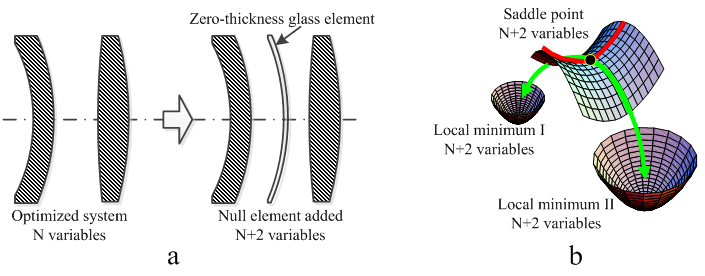
\includegraphics[scale=0.68]{FigSPCDemo.png}
    \caption{Illustration of SPC. (a) SPC with insertion of a zero-thickness glass meniscus. (b) A Morse index one saddle point in the 2D case.}
    \label{fig:SPCdemo}
\end{figure}

The pair of surfaces with equal curvatures can be either a zero-thickness lens added to the old minimum or a zero-thickness air space inside a lens of the old minimum. This added lens or air space will not affect the ray paths, and hence it will not affect the merit function value $MF_0$ of the original system. Therefore, such an element is called a null element. The two added variables are the surface curvatures $c_{N+1}$ and $c_{N+2}$ of the zero-thickness pair of surfaces. For any values of $c_{N+1} = c_{N+2}$ we can therefore write
\begin{equation} \label{eq:1}
    MF(\vec{v_0},c_{N+1},c_{N+2}) = MF_0 \textrm{, for } c_{N+1}=c_{N+2} 
\end{equation} 
where $MF$ is the merit function value of the system after adding the null element, and $\vec{v_0}$ is the vector of all variables of the minimum before insertion, which is kept constant.

In order to find the values of the null element curvatures for which the resulting system is an SP we must find the zeros of the partial derivative of the merit function with respect to the curvature of the null element. In a nutshell, the partial derivatives of the merit function with respect to the old optimization variables remain unchanged, hence they are all zero. Only the derivatives with respect to the new variables need to be considered
for finding the SP. In fact, because these two curvatures are not independent, annulling one of them is sufficient \cite{MVTurnhoutSPC15}. Therefore, if we denote $c_{N+1} = c_s$ to find curvature values for which the system is an SP we look for curvature values cs that satisfy the condition
\begin{equation} \label{eq:2}
    \frac{\partial}{\partial{c_s}} MF(\vec{v_0},c_s,c_{N+2}) \rvert_{c_{N+2}=c_s} = 0
\end{equation}
We solve Equation \ref{eq:2} with a numerical scan programmed in the macro language of CODEV. Since only two variables were added to the original minimum, the MI of this critical point cannot be larger than two. In all cases we have examined so far, the critical points we have found with SPC are only MI one SPs. Figure \ref{fig:SPCscan} shows an example of an SPC scan. There are four zero crossings in Figure \ref{fig:SPCscan}(b) indicating that four SPs are found. When the SPs are found, initial systems for subsequent local optimization can be obtained by choosing for each zero crossing in Figure \ref{fig:SPCscan}(b) two points, one to the left, one to the right of the crossing point. Local optimization, using, e.g., a damped-least square (DLS) algorithm, will then lead to two minimums, one on each side of the “saddle,” as shown in Fig \ref{fig:SPCdemo}(b). To obtain the broadest variety of new minimums with SPC, in general both zero-thickness lenses and zero-thickness airspaces may be necessary. For simple systems, there are examples of minimums that can be obtained with one of these two types of null elements but not with the other one. Finding the saddle points is in principle much less time consuming than DLS optimization, because it only involves the evaluation of the derivative of the MF for the 1D sequence of scan points according to Equation \ref{eq:2}, whereas local optimization involves many iterations where a Jacobian matrix is evaluated. The zero-thickness condition for the null element is not a severe limitation, as it may seem, because in the resulting minimums the distances between the surfaces (and the glass of the new lens) can be easily changed as desired. At this stage other parameters of the new lens (thickness, aspheric coefficients, etc.) can be made variable.

\begin{figure}[h!]
    \centering
    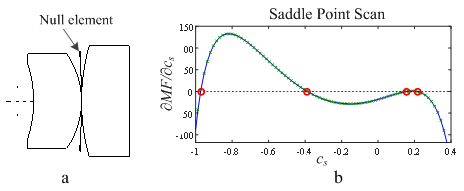
\includegraphics[scale=0.8]{SPCscan}
    \caption{Example of an SPC scan. (a) The insertion of a glass null element between two lenses of a known minimum. (b) The SPC scan finds four saddle points in this search. The red circles indicate the corresponding values of the null element curvatures.}
    \label{fig:SPCscan}
\end{figure}


SPC special should be briefly explained here. 

%%%%%%%%%%%%%%%%%%%%%%%%%%%%%%%%%%%%%%%% SPC intermediate %%%%%%%%%%%%%%%%%%%%%%%%%%%%%%%%%%%%%%%%%%%%%%%
\section{Title Page}

\dropcap{T}{he} title pages are defined in \texttt{title/title.tex}, which you will have to modify according to your needs. Note that these pages are subject to the requirements of the \emph{promotieregelement} and cannot be changed at will. Apart from the names and dates, most of the Dutch text is dictated literally.

Since the thesis title and name of the author appear several times throughout the document (on the title page, but also in, \emph{e.g.}, the preface and cv), special commands are provided so they only have to be specified once. The title (and optional subtitle) can be specified with

\begin{quote}
\texttt{\textbackslash title[Optional subtitle]\{Title\}}
\end{quote}
The name of the author is specified with
\begin{quote}
\texttt{\textbackslash author\{First name\}\{Last name\}}
\end{quote}
Note that the first and last name are separate arguments, since they may be printed in different font shapes. The \texttt{\textbackslash title} and \texttt{\textbackslash author} commands also ensure that the title and author appear in the metadata of the final PDF.

See \texttt{title/title.tex} for detailed documentation on the comment and layout of the title pages. Logos of institutes that have contributed financially to the dissertation may be included on reverse side of the title page. A few example logos can be found in the \texttt{title/logos} folder.

\section{Chapters}

\dropcap{E}{ach} chapter has its own file. For example, the \LaTeX{} source of this chapter can be found in \texttt{chapter-1.tex}. A chapter starts with the command

\begin{quote}
\texttt{\textbackslash chapter\{Chapter title\}}
\end{quote}
This starts a new page, prints the chapter number and title and adds a link in the table of contents. If the title is very long, it may be desirable to use a shorter version in the page headers and the table of contents. This can be achieved by specifying the short title in brackets:

\begin{quote}
\texttt{\textbackslash chapter[Short title]\{Very long title with many words which could not possibly fit on one line\}}
\end{quote}
Unnumbered chapters, such as the preface, can be created with \texttt{\textbackslash chapter*\{Chapter title\}}. Such a chapter will not show up in the table of contents or in the page header. To create a table of contents entry anyway, add
\begin{quote}
    \texttt{\textbackslash addcontentsline\{toc\}\{chapter\}\{Chapter title\}}
\end{quote}
after the \texttt{\textbackslash chapter} command. To print the chapter title in the page header, add
\begin{quote}
    \texttt{\textbackslash setheader\{Chapter title\}}
\end{quote}

If (parts of) the chapter have already been published elsewhere, it is customary to add a reference. This can be done with the special unnumbered footnote command \texttt{\textbackslash blfootnote}. For example,

\begin{quote}
\texttt{\textbackslash blfootnote\{Parts of this chapter have been published in Annalen der Physik \textbackslash textbf\{324\}, 289 (1906) \textbackslash cite \{Einstein1906\}.\}}
\end{quote}
generates the footnote at the beginning of this chapter. Because this footnote is unnumbered, the \texttt{hyperref} package may throw a warning, which safely be ignored.

If multiple people have contributed significantly to this chapter, they can be lister with the \texttt{\textbackslash authors} command. This can be followed by a quotation using \texttt{\textbackslash epigraph} as shown above. Finally, it is customary for a dissertation to include an abstract for every chapter (except perhaps the introduction). This can be accomplished with the \texttt{abstract} environment. The abstract should be followed by \texttt{\textbackslash newpage} to start the chapter text on a new page.

In a dissertation, each chapter has its own list of references. These can be generated with the special command \texttt{\textbackslash references\{dissertation\}} from \texttt{dissertation.bib} at the end of the chapter. Note that this means that you need to run a command like \texttt{bibtex chapter-1/chapter-1} for each chapter. The bibliography style is specified in \texttt{dissertation.bst}, which is a modified version of \texttt{apsrev4-1.bst} (from REVTeX) designed to also display the titles of referenced articles. The template will automatically generate clickable hyperlinks if a URL or DOI (digital object identifier) is present for the reference. Although it is possible to manage the bibliography by hand, we recommend using EndNote (available from Blackboard) or JabRef (available from \url{http://jabref.sourceforge.net/}).

Chapters are subdivided into sections, subsections, subsubsections, and, optionally, paragraphs and subparagraphs. All can have a title, but only sections and subsections are numbered. As with chapters, the numbering can be turned off by using \texttt{\textbackslash section*\{\ldots\}} instead of \texttt{\textbackslash section\{\ldots\}}, and similarly for the subsection.
\section{\textbackslash section\{\ldots\}}
\subsection{\textbackslash subsection\{\ldots\}}
\subsubsection{\textbackslash subsubsection\{\ldots\}}
\paragraph{\textbackslash paragraph\{\ldots\}}
Lorem ipsum dolor sit amet, consectetur adipisicing elit, sed do eiusmod tempor incididunt ut labore et dolore magna aliqua. Ut enim ad minim veniam, quis nostrud exercitation ullamco laboris nisi ut aliquip ex ea commodo consequat. Duis aute irure dolor in reprehenderit in voluptate velit esse cillum dolore eu fugiat nulla pariatur. Excepteur sint occaecat cupidatat non proident, sunt in culpa qui officia deserunt mollit anim id est laborum.

\section{Fonts and Colors}

\dropcap{T}{he} fonts used by this template depend on which version of \LaTeX{} you use. Regular \LaTeX, \emph{i.e.}, if you compile your document with with \texttt{latex}, \texttt{pslatex} or \texttt{pdflatex}, will use Utopia for text, Fourier for math and Latin Modern for sans-serif and monospaced text. However, if you want to adhere to the TU Delft house style, you will need to use \XeLaTeX, as it supports TrueType and OpenType fonts. Compiling with \texttt{xelatex} will use Bookman Old Style for titles, Tahoma for text, Courier New for monospace and Cambria for math. If you want to use \XeLaTeX, but do not want to use the TU Delft house style fonts, you can add the \texttt{nativefonts} option to the document class.

This template supports the use of drop caps, a large colored initial at the beginning of a chapter or section, via the \texttt{\textbackslash dropcap} command:

\begin{quote}
\texttt{\textbackslash dropcap\{L\}\{orem\} ipsum\ldots}
\end{quote}
The first argument is the capital that will be printed on two lines (in the title color), and the second argument is the rest of the word. Depending on the font, the latter may be printed in small caps.

The corporate colors of the TU Delft are cyan, black and white, available, respectively, via \texttt{\textbackslash color\{{\color{tudelft-cyan}tudelft-cyan}\}}, \texttt{\textbackslash color\{{\color{tudelft-black}tudelft-black}\}} (which differs slightly from the default \texttt{black}) and \texttt{\textbackslash color\{tudelft-white\}}. Apart from these three, the house style defines the basic colors
\begin{itemize}
%% Reduce the separation between the items, since this is just a list of words.
\itemsep 0pt
\parskip 0pt
\item\texttt{\color{tudelft-sea-green}tudelft-sea-green},
\item\texttt{\color{tudelft-green}tudelft-green},
\item\texttt{\color{tudelft-dark-blue}tudelft-dark-blue},
\item\texttt{\color{tudelft-purple}tudelft-purple},
\item\texttt{\color{tudelft-turquoise}tudelft-turquoise} and
\item\texttt{\color{tudelft-sky-blue}tudelft-sky-blue},
\end{itemize}
as well as the accent colors
\begin{itemize}
\itemsep 0pt
\parskip 0pt
\item\texttt{\color{tudelft-lavendel}tudelft-lavendel},
\item\texttt{\color{tudelft-orange}tudelft-orange},
\item\texttt{\color{tudelft-warm-purple}tudelft-warm-purple},
\item\texttt{\color{tudelft-fuchsia}tudelft-fuchsia},
\item\texttt{\color{tudelft-bright-green}tudelft-bright-green} and
\item\texttt{\color{tudelft-yellow}tudelft-yellow}.
\end{itemize}

\references{dissertation}

